% Options for packages loaded elsewhere
\PassOptionsToPackage{unicode}{hyperref}
\PassOptionsToPackage{hyphens}{url}
\PassOptionsToPackage{dvipsnames,svgnames*,x11names*}{xcolor}
%
\documentclass[12pt]{article}
\usepackage{lmodern}
\usepackage{amssymb,amsmath}
\usepackage{ifxetex,ifluatex}
\ifnum 0\ifxetex 1\fi\ifluatex 1\fi=0 % if pdftex
  \usepackage[T1]{fontenc}
  \usepackage[utf8]{inputenc}
  \usepackage{textcomp} % provide euro and other symbols
\else % if luatex or xetex
  \usepackage{unicode-math}
  \defaultfontfeatures{Scale=MatchLowercase}
  \defaultfontfeatures[\rmfamily]{Ligatures=TeX,Scale=1}
\fi
% Use upquote if available, for straight quotes in verbatim environments
\IfFileExists{upquote.sty}{\usepackage{upquote}}{}
\IfFileExists{microtype.sty}{% use microtype if available
  \usepackage[]{microtype}
  \UseMicrotypeSet[protrusion]{basicmath} % disable protrusion for tt fonts
}{}
\makeatletter
\@ifundefined{KOMAClassName}{% if non-KOMA class
  \IfFileExists{parskip.sty}{%
    \usepackage{parskip}
  }{% else
    \setlength{\parindent}{0pt}
    \setlength{\parskip}{6pt plus 2pt minus 1pt}}
}{% if KOMA class
  \KOMAoptions{parskip=half}}
\makeatother
\usepackage{xcolor}
\IfFileExists{xurl.sty}{\usepackage{xurl}}{} % add URL line breaks if available
\IfFileExists{bookmark.sty}{\usepackage{bookmark}}{\usepackage{hyperref}}
\hypersetup{
  pdftitle={Connecting the Popularity Adjusted Block Model to the Generalized Random Dot Product Graph for Community Detection and Parameter Estimation},
  colorlinks=true,
  linkcolor=Maroon,
  filecolor=Maroon,
  citecolor=Blue,
  urlcolor=blue,
  pdfcreator={LaTeX via pandoc}}
\urlstyle{same} % disable monospaced font for URLs
%\usepackage[margin=1in]{geometry}
\usepackage{graphicx,grffile}
\def\spacingset#1{\renewcommand{\baselinestretch}%
{#1}\small\normalsize} \spacingset{1}

\makeatletter
\def\maxwidth{\ifdim\Gin@nat@width>\linewidth\linewidth\else\Gin@nat@width\fi}
\def\maxheight{\ifdim\Gin@nat@height>\textheight\textheight\else\Gin@nat@height\fi}
\makeatother
% Scale images if necessary, so that they will not overflow the page
% margins by default, and it is still possible to overwrite the defaults
% using explicit options in \includegraphics[width, height, ...]{}
\setkeys{Gin}{width=\maxwidth,height=\maxheight,keepaspectratio}
% Set default figure placement to htbp
\makeatletter
\def\fps@figure{htbp}
\makeatother
\setlength{\emergencystretch}{3em} % prevent overfull lines
\providecommand{\tightlist}{%
  \setlength{\itemsep}{0pt}\setlength{\parskip}{0pt}}
\setcounter{secnumdepth}{5}
\usepackage{float}
\usepackage{mathtools}
\usepackage{natbib}
\usepackage{parskip}
\usepackage[linesnumbered,ruled,vlined]{algorithm2e}
\setcitestyle{numbers,square,comma}
\usepackage{verbatim}
\usepackage{amsthm}
\usepackage{comment}
\usepackage[]{natbib}
\bibliographystyle{plainnat}
\addtolength{\oddsidemargin}{-.5in}%
\addtolength{\evensidemargin}{-.5in}%
\addtolength{\textwidth}{1in}%
\addtolength{\textheight}{1.3in}%
\addtolength{\topmargin}{-.8in}%

\title{Connecting the Popularity Adjusted Block Model to the Generalized Random
Dot Product Graph for Community Detection and Parameter Estimation}
\author{}
\date{\vspace{-2.5em}}

\begin{document}
\maketitle
\begin{abstract}
We connect two random graph models, the Popularity Adjusted Block Model
(PABM) and the Generalized Random Dot Product Graph (GRDPG),
demonstrating that a PABM is a GRDPG in which communities correspond to
certain mutually orthogonal subspaces of latent positions. This insight
leads to the construction of improved algorithms for community detection
and parameter estimation with PABM. Using established asymptotic
properties of Adjacency Spectral Embedding (ASE) for GRDPG, we derive
asymptotic properties of these algorithms, including algorithms that
rely on Sparse Subspace Clustering (SSC). We illustrate these properties
via simulation.
\end{abstract}

\providecommand{\tightlist}{%
  \setlength{\itemsep}{0pt}\setlength{\parskip}{0pt}}
\newcommand{\diag}{\text{diag}}
\newcommand{\tr}{\text{Tr}}
\newcommand{\blockdiag}{\text{blockdiag}}
\newcommand{\indep}{\stackrel{\text{indep}}{\sim}}
\newcommand{\iid}{\stackrel{\text{iid}}{\sim}}
\newcommand{\Bernoulli}{\text{Bernoulli}}
\newcommand{\Betadist}{\text{Beta}}
\newcommand{\BG}{\text{BernoulliGraph}}
\newcommand{\PABM}{\text{PABM}}
\newcommand{\RDPG}{\text{RDPG}}
\newcommand{\GRDPG}{\text{GRDPG}}
\newcommand{\Multinomial}{\text{Multinomial}}
\newtheorem{definition}{Definition}
\newtheorem{theorem}{Theorem}
\newtheorem{lemma}{Lemma}
\theoremstyle{remark}
\newtheorem*{remark}{Remark}
\theoremstyle{definition}
\newtheorem*{example}{Example}
\newpage
\spacingset{1.5} % DON'T change the spacing!

\hypertarget{introduction}{%
\section{Introduction}\label{introduction}}

Statistical analysis on graphs or networks often involves the
partitioning of a graph into disconnected subgraphs or clusters. This is
often motivated by the assumption that there exist underlying and
unobserved communities to which each vertex of the graph belongs, and
edges between pairs of vertices are determined by drawing from a
probability distribution based on the community relationships between
each pair. The goal of this analysis then is population community
detection, or the recovery of the true underlying community labels for
each vertex, up to permutation, with some additional parameter
estimation being of possible interest, assuming some underlying
probability model. One such model is the Stochastic Block Model (SBM),
first proposed by \citet{doi:10.1080/0022250X.1971.9989788}, which
assumes that the edge probability from one vertex to another follows a
Bernoulli distribution with fixed probabilities for each pair of
community labels. Other random graph models have been proposed and
studied, such as the Degree-Corrected Block Model (DCBM), introduced by
\citet{Karrer_2011}, which is a generalization of the SBM. The
Popularity Adjusted Block Model (PABM) was then introduced by
\citet*{307cbeb9b1be48299388437423d94bf1} as a generalization of the
DCBM to address the heterogeneity of edge probabilities within and
between communities while still maintaining distinct community
structure.

The underlying similarity among the SBM, PABM, and other such models is
that they involve a symmetric edge probability matrix
\(P \in [0, 1]^{n \times n}\) where \(n\) is the number of vertices in
the graph. An undirected and unweighted graph is then drawn from this
edge probability matrix such that the existence of an edge between each
pair of vertices \(i\) and \(j\) is given by
\(\text{Bernoulli}(P_{ij})\). For example, for the SBM with two
communities for which the within-community edge probability is \(\xi\)
and the between-community edge probability is \(\eta\), the entries of
\(P\) consist of \(P_{ij} = \xi\) if \(i\) and \(j\) are in the same
community and \(i \neq j\), \(P_{ij} = \eta\) if \(i\) and \(j\) belong
to separate communities, and \(P_{ii} = 0\).

The Random Dot Product Graph (RDPG) model proposed by
\citet*{10.1007/978-3-540-77004-6_11} is another graph model with
Bernoulli edge probabilities. Under this model, each vertex of the graph
can be represented by a point in some latent space such that the edge
probability between any pair of vertices is given by their corresponding
dot product in the latent space, i.e., given a latent positions
\(x_1, ..., x_n \in \mathbb{R}^d\), the edge probability matrix is
\(P = X X^\top\) where
\(X = \begin{bmatrix} x_1 & \cdots & x_n \end{bmatrix}^\top\). The assortative
SBM is equivalent to a special case of the RDPG for which all vertices
of a given community share the same position in the latent space
\cite{lyzinski2014}. It has also been shown that similar random graph
models, including the DCBM, can be represented in a similar fashion
\cite{lyzinski2014, rubindelanchy2017consistency}. An analogous
property exists for the PABM, not for the RDPG model but the
\emph{Generalized} Random Dot Product Graph (GRDPG) model, which is an
extension of the RDPG to allow edge probability matrices that are not positive
semidefinite. This relationship will be explored in this paper and exploited to
construct algorithms for community detection and parameter estimation for the
PABM.

\hypertarget{notation}{%
\subsection{Notation and Scope}\label{notation}}

Let $G = (V, E)$ be an unweighted, undirected, and hollow graph with vertex set $V$ ($|V| = n$) and edge set $E$. $A \in \{0, 1\}^{n \times n}$ represents the adjacency matrix of $G$ such that $A_{ij} = 1$ if there exists an edge between vertices $i$ and $j$ and $0$ otherwise. Because $G$ is symmetric and hollow,
$A_{ij} = A_{ji}$ and $A_{ii} = 0$ for each $i, j \in [n]$. We further restrict our analyses to Bernoulli graphs. Let $P \in [0, 1]^{n \times n}$ be a symmetric matrix of edge probabilities. Graph $G$ is sampled from $P$ by drawing $A_{ij} \indep \Bernoulli(P_{ij})$ for each $1 \leq i < j \leq n$  (setting $A_{ji} = A_{ij}$ and $A_{ii} = 0$). We denote $A \sim \BG(P)$ as graph with adjacency matrix $A$ sampled from edge probability matrix $P$ in this manner. If each vertex has a hidden label in $[K]$, they are denoted as $z_1, ..., z_n$. Finally, we denote $X = \begin{bmatrix} x_1 & \cdots & x_n \end{bmatrix}^\top \in \mathbb{R}^{n \times d}$ as the collection of $n$ latent vectors $x_1, ..., x_n \in \mathbb{R}^d$.

\hypertarget{connecting-the-popularity-adjusted-block-model-to-the-generalized-random-dot-product-graph}{%
\section{Connecting the Popularity Adjusted Block Model to the
Generalized Random Dot Product
Graph}\label{connecting-the-popularity-adjusted-block-model-to-the-generalized-random-dot-product-graph}}

In this section, we show that the PABM is a special case of the GRDPG, i.e.,
graph $G$ drawn from the PABM can be represented by a collection of latent
vectors in Euclidean space. We further show that the latent configuration that
induces the PABM consists of orthogonal subspaces with each subspace
corresponding to a community.

\hypertarget{the-popularity-adjusted-block-model-and-the-generalized-random-dot-product-graph}{%
\subsection{The Popularity Adjusted Block Model and the Generalized
Random Dot Product
Graph}\label{the-popularity-adjusted-block-model-and-the-generalized-random-dot-product-graph}}

\begin{definition}[Popularity Adjusted Block Model]
\label{pabm}
Let $P \in [0, 1]^{n \times n}$ be a symmetric edge probability matrix for a
graph $G = (V, E)$ with adjacency matrix $A$ such that $A \sim \BG(P)$.
Let each vertex have a community label between $1$ and $K$.
Then $G$ is drawn from a Popularity Adjusted Block Model if
each vertex has $K$ popularity parameters that describe its affinity
toward each of the $K$ communities, i.e., vertex $i$ has popularity parameters
$\lambda_{i1}, ..., \lambda_{iK}$, and
each $P_ij = \lambda_{i z_j} \lambda_{j z_i}$.

Another characterization of the PABM is as follows.
Let the rows and columns of $P$ be arranged by community label
such that $n_k \times n_l$ block $P^{(kl)}$
describes the edge probabilities between vertices in communities
$k$ and $l$ ($P^{(lk)} = (P^{(kl)})^\top$).
If each block $P^{(kl)}$ can be written as the outer product of two vectors:

\begin{equation} \label{eq:pabm}
  P^{(kl)} = \lambda^{(kl)} (\lambda^{(lk)})^\top
\end{equation}

for a set of $K^2$ popularity vectors $\{\lambda^{(st)}\}_{s, t = 1}^K$ where each
$\lambda^{(st)}$ is a column vector of dimension $n_s$, then graph $G$ is drawn from a PABM with parameters $\{\lambda^{(st)}\}_K$ if its its corresponding adjacency matrix $A \sim \BG(P)$.
\end{definition}

We will use the notation \(A \sim \PABM(\{\lambda^{(kl)}\}_K)\) to denote
a random adjacency matrix \(A\) drawn from a PABM with parameters
\(\lambda^{(kl)}\) consisting of \(K\) underlying communities.

\begin{definition}[Generalized Random Dot Product Graph]
\label{grdpg}
Let graph $G = (V, E)$ be drawn as $A \sim \BG(P)$.
If $\exists X \in \mathbb{R}^{n \times d}$ such that

\begin{equation} \label{eq:grdpg}
  P = X I_{p,q} X^\top
\end{equation}

for some $d, p, q \in \mathbb{N}$ and $p + q = d$, then
$G$ is drawn from the Generalized Random Dot Product Graph with latent positions $x_1, ..., x_n \in \mathbb{R}^d$ and signature $(p, q)$.
\end{definition}

We will use the notation \(A \sim \GRDPG_{p,q}(X)\) to denote a random
adjacency matrix \(A\) drawn from latent positions \(X\) and signature
\((p, q)\). If instead of fixed latent positions, they are drawn $X_1, ..., X_n \iid F$, we denote the GRDPG as $(A, X) \sim \GRDPG_{p,q}(F, n)$.

\begin{definition}[Indefinite Orthogonal Group]
The indefinite orthogonal group with signature $(p, q)$ is
the set $\{Q \in \mathbb{R}^{d \times d} : Q I_{p, q} Q^{\top} = I_{p, q}\}$,
denoted as $\mathbb{O}(p, q)$.
\end{definition}

\begin{remark}
Like the RDPG, the latent positions of a GRDPG are not unique
\cite{rubindelanchy2017statistical}.
More specifically, if $P_{ij} = x_i^\top I_{p, q} x_j$, then we also have for any
$Q \in \mathbb{O}(p, q)$,
$(Q x_i)^\top I_{p, q} (Q x_j) = x_i^\top (Q^\top I_{p, q} Q) x_j =
x_i^\top I_{p, q} x_j = P_{ij}$.
Unlike in the RDPG case, transforming the latent positions via multiplication
by $Q \in \mathbb{O}(p, q)$ does not necessarily maintain interpoint angles or
distances.
\end{remark}

\hypertarget{connecting-the-pabm-to-the-grdpg}{%
\subsection{Connecting the PABM to the
GRDPG}\label{connecting-the-pabm-to-the-grdpg}}

\begin{theorem}[Connecting the PABM to the GRDPG for $K = 2$]
\label{theorem1}
Let
$$X = \begin{bmatrix}
\lambda^{(11)} & \lambda^{(12)} & 0 & 0 \\
0 & 0 & \lambda^{(21)} & \lambda^{(22)}
\end{bmatrix} \quad \text{and} \quad
U = \begin{bmatrix} 1 & 0 & 0 & 0 \\
0 & 0 & 1 / \sqrt{2} & 1 / \sqrt{2} \\
0 & 0 & 1 / \sqrt{2} & - 1 / \sqrt{2} \\
0 & 1 & 0 & 0 \end{bmatrix},$$
where the $\{\lambda^{(kl)}\}$ are as defined in Definition 1.
Then $A \sim \mathrm{GRDPG}_{3, 1}(X U)$ and $B \sim \mathrm{PABM}(\{(\lambda^{(kl)}\})$ are
identically distributed.
\end{theorem}

\begin{theorem}[Generalization to $K > 2$]
\label{theorem2}
There exists a block diagonal matrix
$X \in \mathbb{R}^{n \times K^2}$ defined by PABM parameters
$\{\lambda^{(kl)}\}_K$ and orthonormal matrix
$U \in \mathbb{R}^{K^2 \times K^2}$ that is fixed
for each $K$ such that $A \sim GRDPG_{K (K+1) / 2, K (K-1) / 2}(XU)$ and
$A \sim PABM(\{(\lambda^{(kl)}\})_K)$ are equivalent.
\end{theorem}

\begin{proof}
First define the following matrices from $\{\lambda^{(kl)}\}_K$:
\begin{gather}
\label{eq:xy}
\Lambda^{(k)} = \begin{bmatrix} \lambda^{(k,1)} \mid \cdots \mid \lambda^{(k, K)} \end{bmatrix}
\in \mathbb{R}^{n_k \times K}, \quad
X = \text{blockdiag}(\Lambda^{(1)}, \dots, \Lambda^{(K)}) \in
\mathbb{R}^{n \times K^2} \\
L^{(k)} = \text{blockdiag}(\lambda^{(1k)}, \dots, \lambda^{(Kk)}) \in
\mathbb{R}^{n \times K}, \quad
Y = \begin{bmatrix} L^{(1)} \mid \cdots \mid L^{(K)} \end{bmatrix} \in
\mathbb{R}^{n \times K^2}.
\end{gather}
We then have $P = X Y^\top$. Similar to the $K = 2$ case, we have $Y = X \Pi$ for a permutation matrix
$\Pi$, resulting in $P = X \Pi X^\top$.
The permutation described by $\Pi$ has $K$ fixed points, which correspond to
$K$ eigenvalues equal to $1$ with corresponding eigenvectors $e_k$ where
$k = r (K + 1) + 1$ for $r = 0, ..., K - 1$. It also has
$\binom{K}{2} = K (K - 1) / 2$ cycles of order $2$. Each cycle corresponds to
a pair of eigenvalues $+1$ and $-1$ and a pair of eigenvectors
$(e_s + e_t) / \sqrt{2}$ and $(e_s - e_t) / \sqrt{2}$.

Then $\Pi$ has $p = K (K + 1) / 2$ eigenvalues equal to $1$ and $q = K (K - 1) / 2$
eigenvalues equal to $-1$. We therefore have
\begin{equation} \label{eq:permutation}
\Pi = U I_{K (K + 1) / 2, K (K - 1) / 2} U^\top
\end{equation}
where $U$ is a $K^2 \times K^2$ orthogonal matrix. The edge probability matrix can then be written as
\begin{equation} \label{eq:pabm-grdpg}
P = X U I_{p, q} (X U)^\top
\end{equation}
% \begin{equation} \label{eq:p}
% p = K (K + 1) / 2
% \end{equation}
% \begin{equation} \label{eq:q}
% q = K (K - 1) / 2
% \end{equation}
We can therefore describe the PABM with $K$ communities as a GRDPG with latent
positions $X U$ and signature $(p,q) = \bigl( \tfrac{1}{2} K (K + 1) ,
\tfrac{1}{2} K (K - 1)\bigr)$.
\end{proof}

\begin{example}[$K = 3$] Using the same notation as in Theorem
  \ref{theorem2}, we can define
\begin{gather*}
X = \begin{bmatrix}
\lambda^{(11)} & \lambda^{(12)} & \lambda^{(13)} & 0 & 0 & 0 & 0 & 0 & 0 \\
0 & 0 & 0 & \lambda^{(21)} & \lambda^{(22)} & \lambda^{(23)} & 0 & 0 & 0 \\
0 & 0 & 0 & 0 & 0 & 0 & \lambda^{(31)} & \lambda^{(32)} & \lambda^{(33)}
\end{bmatrix}, \\
Y = \begin{bmatrix}
\lambda^{(11)} & 0 & 0 & \lambda^{(12)} & 0 & 0 & \lambda^{(13)} & 0 & 0 \\
0 & \lambda^{(21)} & 0 & 0 & \lambda^{(22)} & 0 & 0 & \lambda^{(23)} & 0 \\
0 & 0 & \lambda^{(31)} & 0 & 0 & \lambda^{(32)} & 0 & 0 & \lambda^{(33)}
\end{bmatrix}.
\end{gather*}
Then $Y = X \Pi$ and $P = X Y^{\top}$ where $\Pi$ is a permutation matrix of
the form
$$\Pi = \begin{bmatrix}
1 & 0 & 0 & 0 & 0 & 0 & 0 & 0 & 0 \\
0 & 0 & 0 & 1 & 0 & 0 & 0 & 0 & 0 \\
0 & 0 & 0 & 0 & 0 & 0 & 1 & 0 & 0 \\
0 & 1 & 0 & 0 & 0 & 0 & 0 & 0 & 0 \\
0 & 0 & 0 & 0 & 1 & 0 & 0 & 0 & 0 \\
0 & 0 & 0 & 0 & 0 & 0 & 0 & 1 & 0 \\
0 & 0 & 1 & 0 & 0 & 0 & 0 & 0 & 0 \\
0 & 0 & 0 & 0 & 0 & 1 & 0 & 0 & 0 \\
0 & 0 & 0 & 0 & 0 & 0 & 0 & 0 & 1
\end{bmatrix}.$$
The matrix $\Pi$ corresponds to a permutation of $\{1,2,\dots,9\}$
with the following decomposition.
\begin{enumerate}
\item Positions 1, 5, 9 are fixed.
\item There are three cycles of length 2, namely $(2, 4)$, $(3, 7)$, and $(6, 8)$.
\end{enumerate}
We can therefore write $\Pi$ as $\Pi = U I_{6, 3} U^\top$ where the first three
columns of $U$ consist of $e_1$, $e_5$, and $e_9$ corresponding to the fixed
positions $1$, $5$, and $9$, the next three columns consist of eigenvectors
$(e_k + e_l) / \sqrt{2}$, and the last three columns consist of eigenvectors
$(e_k - e_l) / \sqrt{2}$, where pairs $(k, l)$ correspond to the cycles of
order 2 described above.

The matrix $P$ can then be written as a generalized random dot product
graph where the latent positions are the rows of the matrix
$$XU = \begin{bmatrix}
  \lambda^{(11)} & 0 & 0 &
  \lambda^{(12)} / \sqrt{2} & \lambda^{(13)} / \sqrt{2} & 0 &
  \lambda^{(12)} / \sqrt{2} & \lambda^{(13)} / \sqrt{2} & 0 \\
  0 & \lambda^{(22)} & 0 &
  \lambda^{(21)} / \sqrt{2} & 0 & \lambda^{(23)} / \sqrt{2} &
  -\lambda^{(21)} / \sqrt{2} & 0 & \lambda^{(23)} / \sqrt{2} \\
  0 & 0 & \lambda^{(33)} &
  0 & \lambda^{(31)} / \sqrt{2} & \lambda^{(32)} / \sqrt{2} &
  0 & -\lambda^{(31)} / \sqrt{2} & -\lambda^{(32)} / \sqrt{2}
\end{bmatrix}$$
\end{example}

\hypertarget{methods}{%
\section{Methods}\label{methods}}

Two inference objectives arise from the PABM:

\begin{enumerate}
\def\labelenumi{\arabic{enumi}.}
\tightlist
\item
  Community membership identification (up to permutation).
\item
  Parameter estimation (estimating \(\lambda^{(kl)}\)'s).
\end{enumerate}

In our methods, we assume that \(K\), the number of communities, is
known beforehand and does not require estimation.

\hypertarget{related-work}{%
\subsection{Related work}\label{related-work}}

\citeauthor{307cbeb9b1be48299388437423d94bf1}, who first proposed the
PABM, used Modularity Maximization (MM) and the Extreme Points (EP)
algorithm \cite{le2016} for community detection and parameter
estimation. They were able to show that as the sample size increases,
the proportion of misclassified community labels (up to permutation)
goes to 0.

\citet*{noroozi2019estimation} used Sparse Subspace Clustering (SSC) for
community detection in the PABM. SSC is performed by solving an
optimization problem for each observed point. Given
\(X \in \mathbb{R}^{n \times d}\) with vectors
\(x_i^\top \in \mathbb{R}^d\) as rows of \(X\), the optimization problem
\(c_i = \arg\min_{c} ||c||_1\) subject to \(x_i = X c\) and
\(c^{(i)} = 0\) is solved for each \(i = 1, ..., n\). The solutions are
collected collected into matrix
\(C = \begin{bmatrix} c_1 & \cdots & c_n \end{bmatrix}^\top\) to
construct an affinity matrix \(B = |C| + |C^\top|\). If each \(x_i\) lie
perfectly on one of \(K\) subspaces, \(B\) describes an undirected graph
consisting of \(K\) disjoint subgraphs, i.e., \(B_{ij} = 0\) if
\(x_i, x_j\) are in different subspaces. If \(X\) instead represents
points near \(K\) subspaces with some noise, a final graph partitioning
step may be performed (e.g., edge thresholding or spectral clustering).

In practice, SSC is often performed by solving the LASSO problems

\begin{equation} \label{eq:ssc}
c_i = \arg\min_c \frac{1}{2} ||x_i - X_{-i} c||^2_2 + \lambda ||c||_1
\end{equation}

for some sparsity parameter \(\lambda > 0\). The \(c_i\) vectors are
then collected into \(C\) and \(B\) as before.

\begin{definition}[Subspace Detection Property]
Let $X = \begin{bmatrix} x_1 & \cdots & x_n \end{bmatrix}^\top$ be noisy
points sampled from $K$ subspaces. Let $C$ and $B$ be constructed from the
solutions of LASSO problems as described in (\ref{eq:ssc}). If each column of
$C$ has nonzero norm and $B_{ij} = 0$ $\forall$ $x_i$ and $x_j$ sampled from
different subspaces, then $X$ obeys the subspace detection property.
\end{definition}

\begin{remark}
In practice, a noisy sample $X$ often does not obey the subspace detection
property. In such cases, $B$ is treated as an affinity matrix for a graph which
is then partitioned into $K$ subgraphs to obtain the clustering. On the other
hand, if $X$ does obey the subspace detection property, $B$ describes a graph
with at least $K$ disconnected subgraphs. Ideally, when the subspace detection
property holds, there are exactly $K$ subgraphs which map to each subspace,
but it could be the case that some of the subspaces are represented by
multiple disconnected subgraphs. The subspace detection property is contingent
on choosing a sufficiently large sparsity parameter $\lambda$.
\end{remark}

Theorem \ref{theorem2} suggests that SSC is appropriate for community
detection for the PABM. More precisely, Theorem \ref{theorem2} says that
each community consists of a \(K\)-dimensional subspace, and together
the subspaces lie in \(\mathbb{R}^{K^2}\). The natural approach then is
to perform SSC on the ASE of \(P\) or \(A\).
\citeauthor{noroozi2019estimation} instead applied SSC to \(P\) and
\(A\), foregoing embedding altogether.

Using results from \citet{soltanolkotabi2012}, it can be easily shown
that the subspace detection property holds for \(XU\), which is an ASE
of \(P\). More specifically, if points lie exactly on mutually
orthogonal subspaces, then the subspace detection property will hold
with probability 1, and this is exactly the case for the PABM (Theorem
\ref{theorem2}). Much of our work is then built on
\citeauthor{rubindelanchy2017statistical}, who describe the convergence
behavior of the ASE of \(A\) to the ASE of \(P\), and
\citet{jmlr-v28-wang13}, who show the necessary conditions for the
subspace detection property to hold in noisy cases where the points lie
near subspaces.

\hypertarget{community-detection}{%
\subsection{Community detection}\label{community-detection}}

\begin{algorithm}[t]
  \DontPrintSemicolon
  \SetAlgoLined
  \KwData{Adjacency matrix $A$, number of communities $K$}
  \KwResult{Community assignments $1, ..., K$}
    Compute the eigenvectors of $A$ that correspond to the $K (K+1) / 2$ most
    positive eigenvalues and $K (K-1) / 2$ most negative eigenvalues. Construct
    $V$ using these eigenvectors as its columns.\;
    Compute $B = |n V V^\top|$, applying $|\cdot|$ entry-wise.\;
    Construct graph $G$ using $B$ as its similarity matrix.\;
    Partition $G$ into $K$ disconnected subgraphs
    (e.g., using edge thresholding or spectral clustering).\;
    Map each partition to the community labels $1, ..., K$.\;
  \caption{Orthogonal Spectral Clustering.}
\end{algorithm}

We previously stated one possible set of latent positions that result in
the edge probability matrix of a PABM, \(P = (XU) I_{p, q} (XU)^\top\). If
we have (or can estimate) \(XU\) directly, then both the community
detection and parameter identification problem are trivial since \(U\)
is orthonormal and fixed for each value of \(K\). However, direct
identification or estimation of \(XU\) is not possible
\cite{rubindelanchy2017statistical}.

If we decompose \(P = Z I_{p, q} Z^\top\), then
\(\exists Q \in \mathbb{O}(p, q)\) such that \(XU = Z Q\). Even if we
start with the exact edge probability matrix, we cannot recover the
``original'' latent positions \(XU\). Note that unlike in the case of
the RDPG, \(Q\) is not necessarily an orthogonal matrix. If \(z_i\)'s
are the rows of \(XU\), then
\(||z_i - z_j||^2 \neq ||Q z_i - Q z_j||^2\), and
\(\langle z_i, z_j \rangle \neq \langle Q z_i, Q z_j \rangle\). This
prevents us from using the properties of \(XU\) directly. In particular,
if \(Q \in \mathbb{O}(n)\), then we could use the fact that
\(\langle z_i, z_j \rangle = \langle Q z_i, Q z_j \rangle = 0\) if
vertices \(i\) and \(j\) are in different communities.

The explicit form of \(XU\) represents points in \(\mathbb{R}^{K^2}\)
such that points within each community lie on \(K\)-dimensional
orthogonal subspaces. Multiplication by \(Q \in \mathbb{O}(p, q)\)
removes the orthogonality property but retains the property that each
community is represented by a \(K\)-dimensional subspace. Therefore, the
ASE of \(P\) results in subspaces that correspond to each community,
suggesting the use of SSC. Before exploring SSC, we will first consider
a different approach.

\begin{theorem}
\label{theorem3}
Let $P = V D V^\top$ be the spectral decomposition of the edge probability
matrix. Let $B = n V V^\top$. Then $B_{ij} = 0$ if vertices $i$ and $j$ are
from different communities.
\end{theorem}

Theorem \ref{theorem3} provides perfect community detection given \(P\).
Letting \(|B|\) be the affinity matrix for graph \(G\), \(G\) is
partitioned into at least \(K\) disjoint subgraphs since each of the
\(K\) communities have no edges between them. Similar to the subspace
detection property, it could be the case that some of the communities
are represented by multiple disjoint subgraphs in \(G\), in which case
additional reconstruction is required to identify the communities
exactly.

Using \(A\) instead of \(P\) introduces error, which converges to \(0\)
almost surely:

\begin{theorem}
\label{theorem4}
Let $\hat{B}_n$ with entries $\hat{B}_n^{(ij)}$ be the affinity matrix from OSC
(Alg. 1). Then $\forall$ pairs $(i, j)$ belonging to different communities
and sparsity factor satisfying $n \rho_n = \omega\{(\log n)^{4c}\}$,

\begin{equation} \label{eq:thm4}
\max_{i, j} |n (\hat{v}_n^{(i)})^\top \hat{v}_n^{(j)}| =
O_P \Big( \frac{(\log n)^c}{\sqrt{n \rho_n}} \Big)
\end{equation}

This provides the result that for $i, j$ in different communities,
$\hat{B}_n^{(ij)} \stackrel{a.s.}{\to} 0$.
\end{theorem}

Theorems \ref{theorem2}, \ref{theorem3}, and \ref{theorem4} also provide
a very natural path toward using SSC for community detection for the
PABM. We established in Theorem \ref{theorem2} that an ASE of the edge
probability matrix \(P\) can be constructed such that the communities
lie on mutually orthogonal subspaces, and this property can be recovered
from the eigenvectors of \(P\). Then Theorems \ref{theorem3} and
\ref{theorem4} show that this property holds for the unscaled ASE of
\(A\) drawn from \(P\) as \(n \to \infty\).

\begin{algorithm}[t]
  \DontPrintSemicolon
  \SetAlgoLined
  \caption{Sparse Subspace Clustering using LASSO \cite{jmlr-v28-wang13}.}
  \KwData{Adjacency matrix $A$, number of communities $K$,
  hyperparameter $\lambda$}
  \KwResult{Community assignments $1, ..., K$}
    Find $V$, the matrix of eigenvectors of $A$
    corresponding to the $K (K + 1) / 2$ most positive
    and the $K (K - 1) / 2$ most negative eigenvalues.\;
    Normalize $V \leftarrow \sqrt{n} V$.\;
    \For {$i = 1, ..., n$} {
      Assign $v_i^\top$ as the $i^{th}$ row of $V$.
      Assign $V_{-i} = \begin{bmatrix}
      v_1 & \cdots & v_{i-1} & v_{i+1} & \cdots & v_n \end{bmatrix}^\top$.\;
      Solve the LASSO problem
      $c_i = \arg\min_{\beta}
      \frac{1}{2} ||v_i - V_{-i} \beta||_2^2 + \lambda ||\beta||_1$.\;
      Assign $\tilde{c}_i = \begin{bmatrix}
      c_i^{(1)} & \cdots & c_i^{(i-1)} & 0 & c_i^{(i)} & \cdots & c_i^{(n-1)}
      \end{bmatrix}^\top$ such that the superscript is the index of
      $\tilde{c}_i$.\;
    }
    Assign
    $C = \begin{bmatrix} \tilde{c}_1 & \cdots & \tilde{c}_n \end{bmatrix}$.\;
    Compute the affinity matrix $B = |C| + |C^\top|$.\;
    Construct graph $G$ using $B$ as its similarity matrix.\;
    Partition $G$ into $K$ disconnected subgraphs (e.g., using edge
    thresholding or spectral clustering).\;
    Map each partition to the community labels $1, ..., K$.
\end{algorithm}

\begin{theorem}
\label{theorem5}
Let $P_n$ describe the edge probability matrix of the PABM with
$n$ vertices, and let $A_n \sim \text{Bernoulli}(P_n)$.  Let $\hat{V}_n$ be the
matrix of eigenvectors of $A_n$ corresponding to the $K (K + 1) / 2$ most
positive and $K (K - 1) / 2$ most negative eigenvalues. Then
$\exists \lambda > 0$ and $N \in \mathbb{N}$ such that when $n > N$,
$\sqrt{n} \hat{V}_n$ obeys the subspace detection property with probability 1.
\end{theorem}

\begin{remark}
The proof of Theorem \ref{theorem5} is a direct consequence of Theorem 6
from  \citeauthor{jmlr-v28-wang13} and the fact that the unscaled ASE of
$P_n$ consists of orthogonal subspaces. \citeauthor{jmlr-v28-wang13} assume
that the points in the embedding are all of unit length, and while we apply
this normalization in the simulated examples, it is not strictly necessary
for Theorem \ref{theorem5} due to orthogonality.
\end{remark}

\hypertarget{parameter-estimation}{%
\subsection{Parameter estimation}\label{parameter-estimation}}

For any edge probability matrix \(P\) for the PABM such that the rows
and columns are organized by community, the \(kl\)\textsuperscript{th}
block is an outer product of two vectors, i.e.,
\(P^{(kl)} = \lambda^{(kl)} (\lambda^{(lk)})^\top\). Therefore, given
\(P^{(kl)}\), \(\lambda^{(kl)}\) and \(\lambda^{(lk)}\) are solvable
up to multiplicative constant using singular value
decomposition. More specifically, 
let \(P^{(kl)} = (\sigma^{(kl)})^2 u^{(kl)} (v^{(kl)})^\top\)
be the singular value decomposition of \(P^{(kl)}\).
\(u^{(kl)} \in \mathbb{R}^{n_k}\) and 
\(v^{(kl)} \in \mathbb{R}^{n_l}\) are vectors
and \(\sigma^{(kl)}\) is a scalar. Then \(\lambda^{(kl)} = s_1 u^{(kl)}\)
and \(\lambda^{(lk)} = s_2 v^{(kl)}\) 
for unidentifiable $s_1 s_2 = (\sigma^{(kl)})^2$.
Given the adjacency matrix \(A\)
instead of edge probability matrix \(P\), we can simply use plug-in
estimators by taking the SVD of each $A^{(kl)}$. 
Since each $\lambda^{(kl)}$ is not strictly identifiable,
we instead estimate each $\tilde{\lambda}^{(kl)} = \sigma^{(kl)} u^{(kl)}$. 

\begin{algorithm}[t]
  \DontPrintSemicolon
  \SetAlgoLined
  \caption{PABM parameter estimation.}
  \KwData{Adjacency matrix $A$, community assignments $1, ..., K$}
  \KwResult{PABM parameter estimates $\{\hat{\lambda}^{(kl)}\}_K$.}
  Arrange the rows and columns of $A$ by community such that each 
  $A^{(kl)}$ block consists of estimated edge probabilities between 
  communities $k$ and $l$.\;
  \For {$k, l = 1, ..., K$, $k \leq l$} {
    Compute $A^{(kl)} = U \Sigma V^\top$, the SVD of the $kl^{th}$ 
    block.\;
    Assign $u^{(kl)}$ and $v^{(kl)}$ as the first columns of $U$ and $V$. 
    Assign $(\sigma^{(kl)})^2 \leftarrow \Sigma_{11}$.\;
    Assign $\hat{\lambda}^{(kl)} \leftarrow \pm \sigma^{(kl)} u^{(kl)}$ and 
    $\hat{\lambda}^{(lk)} \leftarrow \pm \sigma^{(kl)} v^{(kl)}$.
  }
\end{algorithm}

\begin{theorem}
\label{theorem6}
Under regularity and sparsity assumptions, given fixed $K$, 

\begin{equation} \label{eq:thm6}
\max_{k, l \in \{1, ..., K\}} 
||\hat{\lambda}^{(kl)} - \lambda^{(kl)}|| = 
O_P \bigg(\frac{(\log n_k)^c}{\sqrt{n_k}} \bigg)
\end{equation}
\end{theorem}

\hypertarget{simulated-examples}{%
\section{Simulated Examples}\label{simulated-examples}}

For each simulation, community labels are drawn from a multinomial
distribution, the popularity vectors \(\{\lambda^{(kl)}\}_K\) are drawn
from two types of joint distributions depending on whether \(k = l\),
the edge probability matrix \(P\) is constructed using the popularity
vectors, and finally an unweighted and undirected adjacency matrix \(A\)
is drawn from \(P\). OSC is then used for community detection, and this
method is compared against SSC \cite{noroozi2019estimation,soltanolkotabi2014}
and MM \cite{igraph}
\cite{307cbeb9b1be48299388437423d94bf1}. True community labels are used
with Algorithm 3 to estimate the popularity vectors
\(\{\lambda^{(kl)}\}_K\), and this method is then compared against an
MLE-based estimator described by \citeauthor{noroozi2019estimation} and
\citeauthor{307cbeb9b1be48299388437423d94bf1}.

Modularity Maximization is NP-hard, so
\citeauthor{307cbeb9b1be48299388437423d94bf1} used the Extreme Points
(EP) algorithm \cite{le2016}, which is \(O(n^{K - 1})\), as a greedy
relaxation of the optimization problem. For these simulations, the
Louvain algorithm was used for modularity maximization,
as \citeauthor{307cbeb9b1be48299388437423d94bf1}'s implementation proved to be
prohibitively computationally expensive for \(K > 2\). For \(K = 2\), it
was verified that the Louvain algorithm produces comparable results
to EP-MM.

Two implementations of SSC are shown here. The first method, denoted as
SSC-A, treats the columns of the adjacency matrix \(A\) as points in
\(\mathbb{R}^n\), as described in \citeauthor{noroozi2019estimation}.
The second method, denoted as SSC-ASE, first embeds \(A\) and then
performs SSC on the embedding, as described in algorithm 2. The sparsity
parameter \(\lambda\) was chosen via a preliminary cross-validation
experiment. For the final clustering step, a Gaussian Mixture Model was
fit on the normalized Laplacian eigenmap of the affinity matrix \(B\).

For comparing methods, we define the community detection error as:

\[L_c(\hat{\sigma}, \sigma; \{v_i\}) =
\min_\pi \sum_i I(\pi \circ \hat{\sigma}(v_i) = \sigma(v_i))\]

where \(\sigma(v_i)\) is the true community label of vertex \(v_i\),
\(\hat{\sigma}(v_i)\) is the predicted label of \(v_i\), and \(\pi\) is
a permutation operator. This is effectively the ``misclustering count''
of clustering function \(\hat{\sigma}\).

We also define two types of parameter estimation error. 
First, we estimate the popularity vectors directly and compute the RMSE. 
In this case, the "true" popularity vectors are derived from 
taking the SVD of each edge probability block $P^{(kl)}$ 
to avoid the unidentifiable multiplicative constants. 

\[\text{RMSE}(\{\hat{\lambda}^{(kl)}\}_K, \{\lambda^{(kl)}\}_K) = 
\sqrt{\frac{1}{n} \sum_{k < l} \min_{s = \pm 1} 
\|s \hat{\lambda}^{(kl)} - \lambda^{(kl)} \|_2^2}\]

We can also avoid the unidentifiable multiplicative constant more directly 
by reconstructing each 
$\hat{P}^{(kl)} = \hat{\lambda}^{(kl)} (\hat{\lambda}^{(lk)})^\top$, 
which we use to define another parameter estimation error. 

\[\text{RMSE}(\hat{P}, P) =
\sum_{k,l} \sqrt{\frac{1}{n_k n_l} \|P^{(kl)} - \hat{P}^{(kl)}\|_F^2}\]

\hypertarget{balanced-communities}{%
\subsection{Balanced communities}\label{balanced-communities}}

In each simulation, community labels \(z_1, ..., z_n\) were drawn from a
multinomial distribution with mixture parameters
\(\{\alpha_1, ..., \alpha_K\}\), then \(\{\lambda^{(kl)}\}_K\) according
to the drawn community labels, \(P\) was constructed using the drawn
\(\{\lambda^{(kl)}\}_K\), and \(A\) was drawn from \(P\) by
\(A_{ij} \indep \Bernoulli(P_{ij})\). Each simulation has
a unique edge probability matrix \(P\).

For these examples, we set the following parameters:

\begin{itemize}
\tightlist
\item
  Number of vertices \(n = 128, 256, 512, 1024, 2048, 4096\)
\item
  Number of underlying communities \(K = 2, 3, 4\)
\item
  Mixture parameters \(\alpha_k = 1 / K\) for \(k = 1, ..., K\), (i.e.,
  each community label has an equal probability of being drawn)
\item
  Community labels
  \(z_k \stackrel{\text{iid}}{\sim} \Multinomial(\alpha_1, ..., \alpha_K)\)
\item
  Within-group popularities
  \(\lambda^{(kk)} \stackrel{\text{iid}}{\sim} \Betadist(2, 1)\)
\item
  Between-group popularities
  \(\lambda^{(kl)} \stackrel{\text{iid}}{\sim} \Betadist(1, 2)\) for
  \(k \neq l\)
\end{itemize}

\(50\) simulations were performed for each \((n, K)\) pair.

\begin{comment}

Fig. \ref{fig:clust_err_k} show that for large $n$, OSC results in
a misclustering rate of 0.

\begin{figure}[H]

{\centering 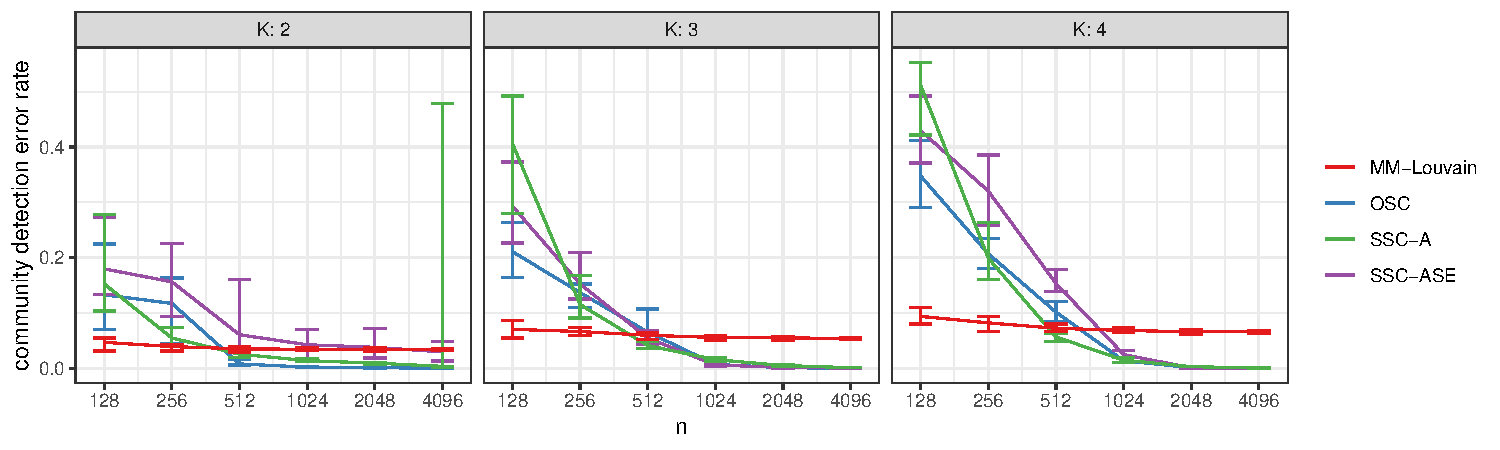
\includegraphics{summary_files/figure-latex/clust_err_k-1}

}

\caption{IQR of community detection error error using OSC (blue) compared against SSC on the ASE of A (purple), MM (red), and SSC on the adjacency matrix (green). Communities are approximately balanced. Simulations were repeated 50 times for each sample size.}\label{fig:clust_err_k}
\end{figure}

Theorem \ref{theorem4} implies that OSC will result in not just in the error
rate converging to 0 but the error *count* as well.
We explore this in Fig. \ref{fig:clust_err_ct_sim}.

\end{comment}

Fig \ref{fig:clust_err_ct_sim} shows OSC's community detection error
going to 0 for large \(n\). SSC on both the embedding and on the
adjacency matrix produces similar results for \(K > 2\). Weaker
performance of SSC for \(K = 2\) can be attributed to the final spectral
clustering step of the affinity matrix. A GMM was fit to the Laplacian
eigenmap, but visual inspection suggests that the communities are not
distributed as a mixture of Gaussians in the eigenmap. While the
subspace detection property is guaranteed for large \(n\), in our
simulations, setting a large enough sparsity parameter for SSC resulted
in more than \(K\) disconnected subgraphs.

\begin{figure}[H]

{\centering 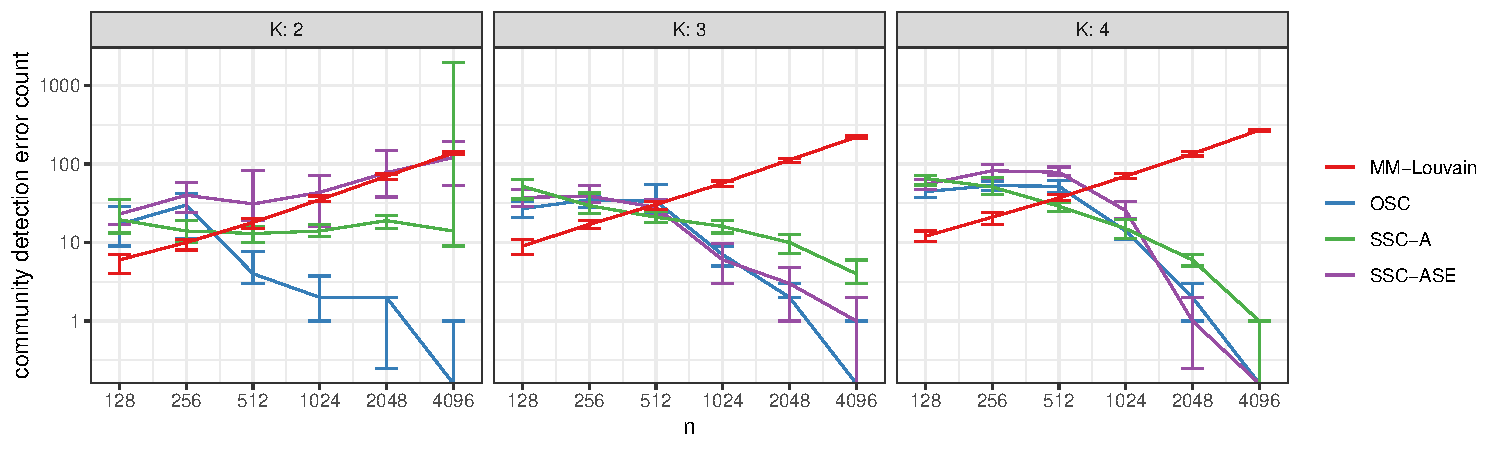
\includegraphics{summary_files/figure-latex/clust_err_ct_sim-1}

}

\caption{Median and IQR of community detection error. Communities are approximately balanced. Simulations were repeated 50 times for each sample size.}\label{fig:clust_err_ct_sim}
\end{figure}

Given ground truth community labels, Algorithm 3 and the MLE-based
plug-in estimators \cite{307cbeb9b1be48299388437423d94bf1} 
perform similarly, with root mean square
error decaying at rate approximately \(n^{-1/2}\).

\begin{figure}[H]

{\centering 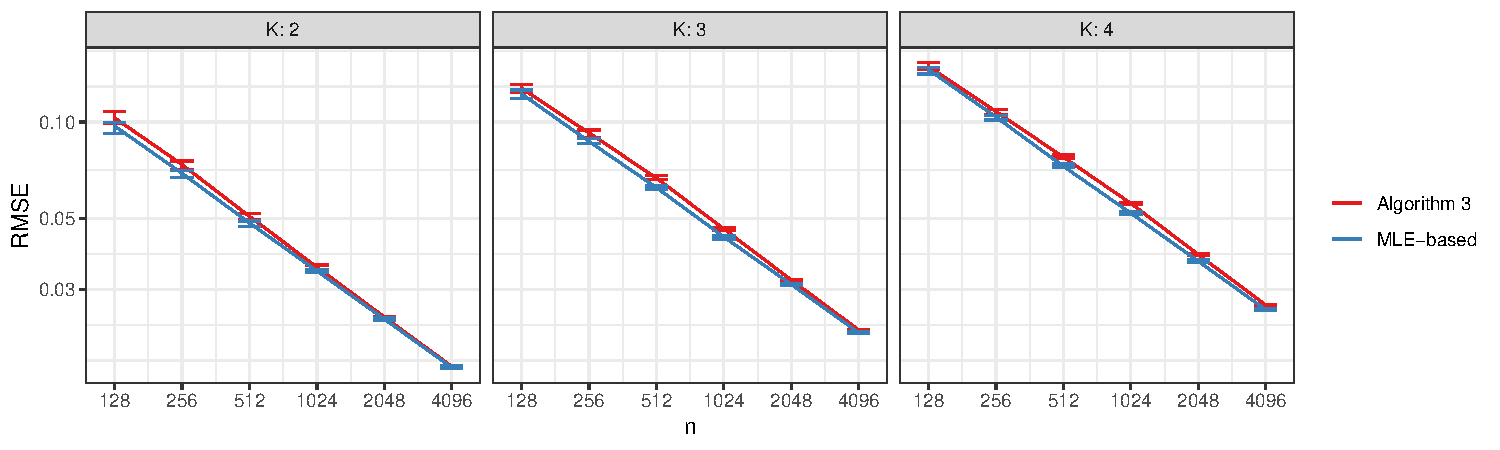
\includegraphics{summary_files/figure-latex/lambda_est_k-1}

}

\caption{Median and IQR RMSE from Algorithm 3 (red) compared against an MLE-based method (blue). Simulations were repeated 50 times for each sample size. Communities were drawn to be approximately balanced.}\label{fig:lambda_est_k}
\end{figure}

\hypertarget{imbalanced-communities}{%
\subsection{Imbalanced communities}\label{imbalanced-communities}}

Simulations performed in this section are similar to those in the
previous section with the exception of the mixture parameters
\(\{\alpha_1, ..., \alpha_K\}\) used to draw community labels from the
multinomial distribution. For these examples, we set the following
parameters:

\begin{itemize}
\tightlist
\item
  Number of vertices \(n = 128, 256, 512, 1024, 2048, 4096\)
\item
  Number of underlying communities \(K = 2, 3, 4\)
\item
  Mixture parameters \(\alpha_k = \frac{k^{-1}}{\sum_{l=1}^K l^{-1}}\)
  for \(k = 1, ..., K\)
\item
  Community labels
  \(z_k \stackrel{\text{iid}}{\sim}Multinomial(\alpha_1, ..., \alpha_K)\)
\item
  Within-group popularities
  \(\lambda^{(kk)} \stackrel{\text{iid}}{\sim}Beta(2, 1)\)
\item
  Between-group popularities
  \(\lambda^{(kl)} \stackrel{\text{iid}}{\sim}Beta(1, 2)\) for
  \(k \neq l\)
\end{itemize}

\(50\) simulations were performed for each \((n, K)\) pair.

\begin{comment}

Fig. \ref{fig:clust_err_k_imba} and \ref{fig:clust_err_ct_sim_imba} show
similar results as in the balanced communities case, with both OSC and
SSC resulting in no misclustered vertices for a
sufficiently large sample size. However, Fig. \ref{fig:lambda_est_k_imba}
suggests that while Algorithm 3 retains $\sqrt{n}$ efficiency, the MLE-based
plug-in estimator is less efficient for this setup.

\begin{figure}[H]

{\centering 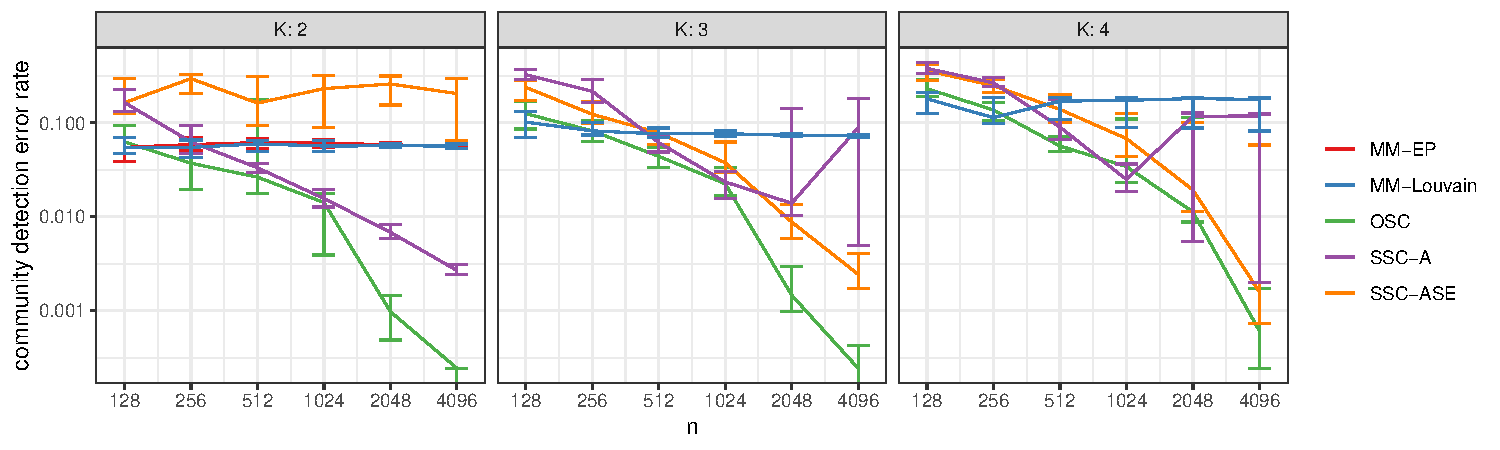
\includegraphics{summary_files/figure-latex/clust_err_k_imba-1}

}

\caption{Median and IQR of community detection error using OSC (blue) compared against SSC on the ASE of A (purple), MM (red), and SSC on the adjacency matrix (green). Communities are imbalanced. Simulations were repeated 50 times for each sample size.}\label{fig:clust_err_k_imba}
\end{figure}

\end{comment}

We again see community detection error trending to 0 for OSC, as well as
for SSC when \(K > 2\) (Fig. \ref{fig:clust_err_ct_sim_imba}). Alg. 3
continues to see \(n^{-1/2}\) decay in parameter estimation error
(\ref{fig:lambda_est_k_imba}).

\begin{figure}[H]

{\centering 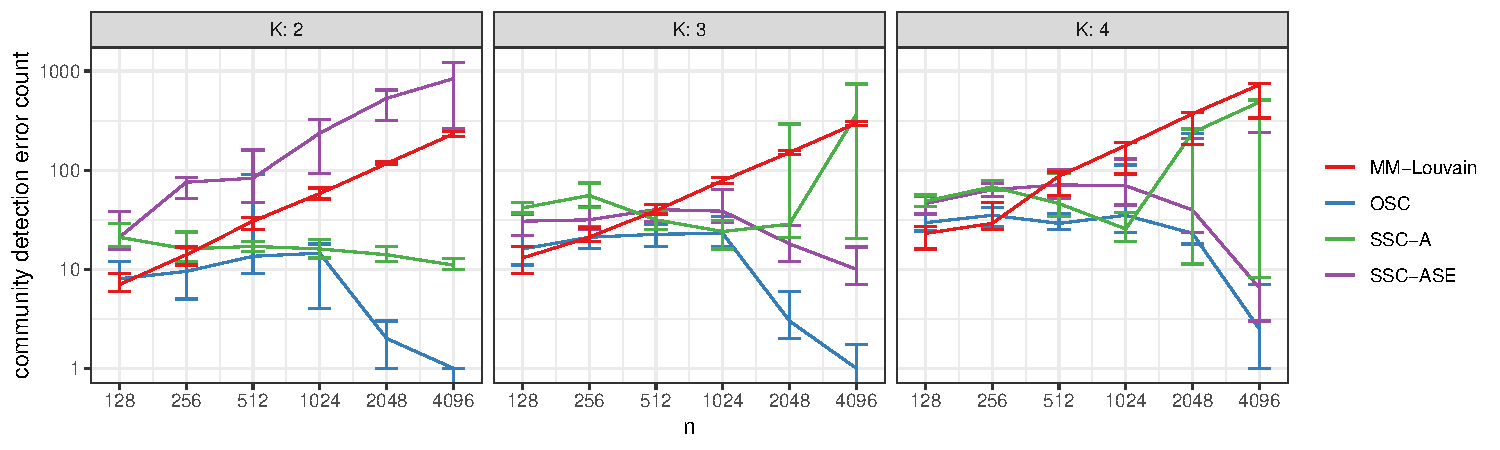
\includegraphics{summary_files/figure-latex/clust_err_ct_sim_imba-1}

}

\caption{Median and IQR of community detection error. Communities are imbalanced. Simulations were repeated 50 times for each sample size.}\label{fig:clust_err_ct_sim_imba}
\end{figure}

\begin{figure}[H]

{\centering 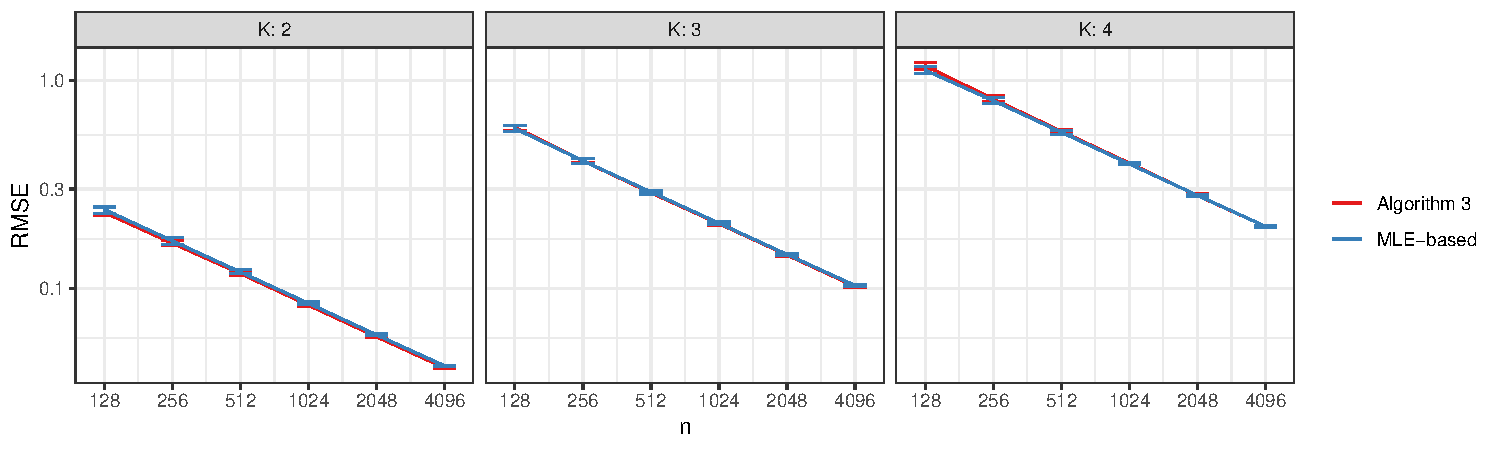
\includegraphics{summary_files/figure-latex/lambda_est_k_imba-1}

}

\caption{Median and IQR RMSE from Algorithm 3 (red) compared against an MLE-based method (blue). Simulations were repeated 50 times for each sample size. Communities were drawn to be imbalanced.}\label{fig:lambda_est_k_imba}
\end{figure}

\begin{comment}

## Additional experiments

Using the same set of parameters for generating $P$ and $A$ as in the
balanced communities examples for $K = 2$, we generated one instance of $A$ for
each $n$ and constructed $B$ according to Algorithm 3 to verify that
as $n \to \infty$, $(\hat{v}_i)^\top \hat{v_j} \stackrel{a.s.}{\to} 0$ for $i, j$
in different clusters. Furthermore, the distribution of these inner products
should be approximately normal.

\begin{figure}[H]

{\centering 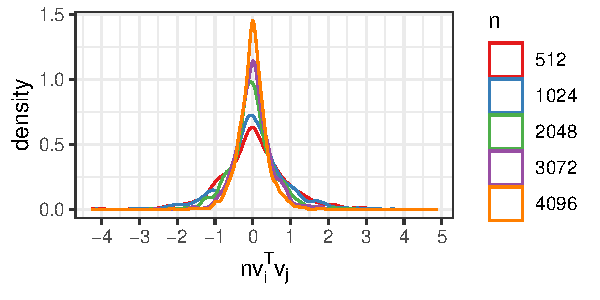
\includegraphics{summary_files/figure-latex/unnamed-chunk-2-1}

}

\caption{Between-cluster inner products of the eigenvectors of $A$ for varying sample sizes.}\label{fig:unnamed-chunk-2}
\end{figure}

\end{comment}

\hypertarget{real-data-examples}{%
\section{Real data examples}\label{real-data-examples}}

In the first real data example, we applied OSC to the Leeds Butterfly
dataset \cite{Wang_2018} consisting of visual similarity measurements
among 832 butterflies across 10 species. The graph was modified to match
the example from \citeauthor{noroozi2019estimation}: Only the 4 most
frequent species were considered, and the similarities were discretized
to \(\{0, 1\}\) via thresholding. Fig. \ref{fig:butterfly} shows a
sorted adjacency matrix sorted by the resultant clustering.

Comparing against the ground truth species labels, OSC achieves an
accuracy of 63\% and an adjusted Rand index of 73\%. In comparison,
\citeauthor{noroozi2019estimation} achieved an adjusted Rand index of
73\% using sparse subspace clustering on the same dataset.

\begin{figure}[H]

{\centering 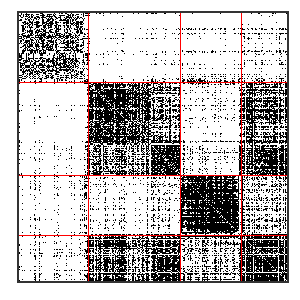
\includegraphics{summary_files/figure-latex/butterfly-1}

}

\caption{Adjacency matrix of the Leeds Butterfly dataset after sorting by the clustering outputted by OSC.}\label{fig:butterfly}
\end{figure}

In the second example, we applied OSC to the British MPs Twitter network
\cite{greene2013producing}, the Political Blogs network
\cite{10.1145/1134271.1134277}, and the DBLP network
\cite{NIPS2009_3855} \cite{10.1007/978-3-642-15880-3_42}. For this data
analysis, we subsetted the data as described by
\citeauthor{307cbeb9b1be48299388437423d94bf1} for their analysis of the
same networks. Our methods underperformed compared to modularity
maximization, although performance is comparable. In addition, OSC's
runtime is much lower than that of modularity maximization.

\begin{table}

\caption{\label{tab:unnamed-chunk-6}Community detection error rates for modularity maximization, sparse subspace clustering,  and OSC.}
\centering
\begin{tabular}[t]{l|r|r|r}
\hline
Network & MM & SSC-ASE & OSC\\
\hline
British MPs & 0.003 & 0.018 & 0.009\\
\hline
Political blogs & 0.050 & 0.196 & 0.062\\
\hline
DBLP & 0.028 & 0.087 & 0.059\\
\hline
\end{tabular}
\end{table}

\begin{figure}[H]

{\centering 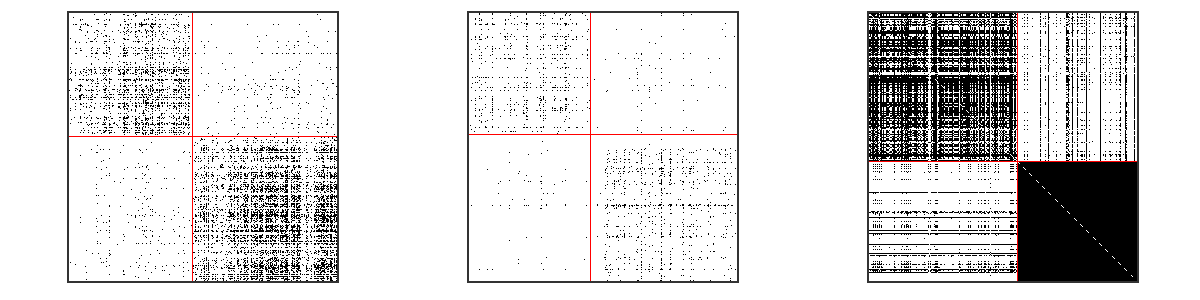
\includegraphics{summary_files/figure-latex/mp-1}

}

\caption{Adjacency matrices of (from left to right) the British MPs, Political Blogs, and DBLP networks after sorting by the clustering outputted by OSC.}\label{fig:mp}
\end{figure}

In the third example, we consider the Karantaka villages data studied by
\citet{DVN/U3BIHX_2013}. For this example, we chose the \texttt{visitgo}
networks from villages 12, 31, and 46 at the household level. The label
of interest is the religious affiliation. The networks were truncated to
religions ``1'' and ``2'', and vertices of degree 0 were removed.

\begin{figure}[H]

{\centering 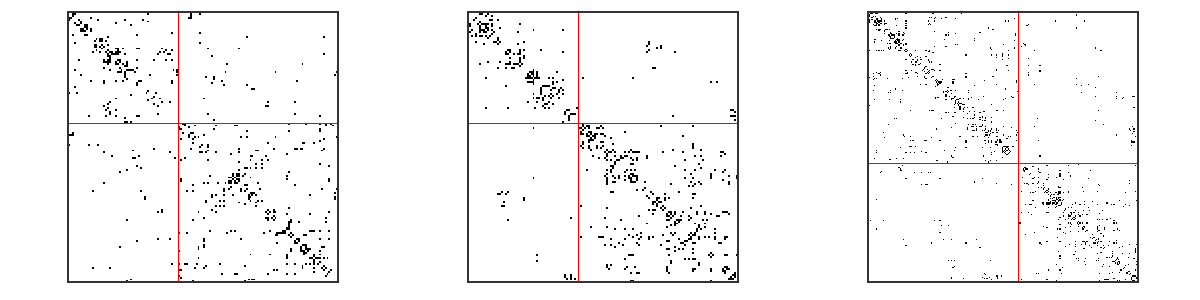
\includegraphics{summary_files/figure-latex/unnamed-chunk-7-1}

}

\caption{Adjacency matrix of the Karnataka villages data, arranged by the clustering produced by OSC (left). The villages studied here are, from left to right, 12, 31, and 46.}\label{fig:unnamed-chunk-7}
\end{figure}

\begin{table}

\caption{\label{tab:unnamed-chunk-8}Community detection error rates for identifying household religion.}
\centering
\begin{tabular}[t]{l|r|r|r}
\hline
Network & MM & SSC-ASE & OSC\\
\hline
Village 12 & 0.270 & 0.291 & 0.227\\
\hline
Village 31 & 0.125 & 0.066 & 0.110\\
\hline
Village 46 & 0.052 & 0.463 & 0.078\\
\hline
\end{tabular}
\end{table}

\hypertarget{discussion}{%
\section{Discussion}\label{discussion}}

This paper shows the connection between the PABM and the GRDPG, namely
that a PABM graph can be represented as a union of orthogonal subspaces
in an embedding under the GRDPG framework. We then exploited this
relationship to develop community detection and parameter estimation
methods. In fact, we can represent any graph with Bernoulli edges as a
GRDPG, and in the PABM case, it turns out that this relationship leads
to a very straightforward applications of previous work from
\citeauthor{rubindelanchy2017statistical},
\citeauthor{soltanolkotabi2012}, and \citeauthor{jmlr-v28-wang13}, which
lead to asymptotically correct solutions with high probability. Similar
methods can be applied for other models, such as the Nested Block Model
\cite{noroozi2021hierarchy}.

\hypertarget{proofs}{%
\section{Proofs}\label{proofs}}

\textbf{Proof of Theorem \ref{theorem1}}. This is given by
straightforward matrix multiplication. It suffices to show that

\[X U I_{3, 1} U^\top X^\top =
\begin{bmatrix}
  \lambda^{(11)} (\lambda^{(11)})^\top & \lambda^{(12)} (\lambda^{(21)})^\top \\
  \lambda^{(21)} (\lambda^{(12)})^\top & \lambda^{(22)} (\lambda^{(22)})^\top
\end{bmatrix}\]

\begin{remark}
While we can just perform the matrix multiplication to show the
equivalence, it is more illustrative to look at a few intermediate steps. Note
that the product of the three inner matrices results in a permutation matrix
with fixed points at positions $1$ and $4$ and a cycle of order 2 swapping
positions $2$ and $3$:

$$U I_{3, 1} U^\top = \begin{bmatrix}
  1 & 0 & 0 & 0 \\
  0 & 0 & 1 & 0 \\
  0 & 1 & 0 & 0 \\
  0 & 0 & 0 & 1
\end{bmatrix} = \Pi$$

Since $U$ is orthonormal and $I_{3, 1}$ is diagonal, $\Pi = U I_{3, 1} U^\top$
is a spectral decomposition of this permutation matrix. Note that the two fixed
points result in eigenvalues of $+1$ with corresponding eigenvectors $e_i$
where $i = 1, 4$ corresponding to the locations of the fixed points, and the
cycle of order two results in two eigenvalues $\pm 1$ with corresponding
eigenvectors $(e_i \pm e_j) / \sqrt{2}$ where $i = 2, j = 3$, pair that is
swapped.
\end{remark}

\begin{lemma}
\label{lemma1}
Let $P = V D V^\top$ be the spectral decomposition of the edge probability
matrix for a PABM. Then $V V^\top = X (X^\top X)^{-1} X^\top$ where $X$ is
defined as in (\ref{eq:xy}).
\end{lemma}

\emph{Proof}. By Theorem 2, \(P = X U I_{p, q} U^\top X^\top\), where
\(X\) is defined as in (\ref{eq:xy}) and $p = K(K+1)/2$ and $q = K(K-1)/2$. % are given by $p =
% K(K+1)/2$ and $q = are defined as
% in equations (\ref{eq:p}) and (\ref{eq:q}).
Alternatively, the spectral
decomposition can be written as
\(P = V D V^\top = V |D|^{1/2} I_{p, q} |D|^{1/2} V^\top\) for the same
\((p, q)\) and \(|\cdot|^{1/2}\) is applied entry-wise. Thus for some
\(Q \in \mathbb{O}(p, q)\),

\[X U Q = V |D|^{1/2}\]

Therefore, using the fact that \(U U^\top = I\) and \(V^\top V = I\),

\[(V |D|^{1/2}) ((V |D|^{1/2})^\top (V |D|^{1/2}))^{-1} (V |D|^{1/2})^\top =
(X U Q) ((X U Q)^\top (X U Q))^{-1} (X U Q)^\top\]

The right-hand side becomes

\[\begin{split}
  (X U Q) ((X U Q)^\top (X U Q))^{-1} (X U Q)^\top &
    = X U Q Q^{-1} U^\top (X^\top X)^{-1}
    U (Q^\top)^{-1} Q^\top U^\top X^\top \\
  & = X U U^\top (X^\top X)^{-1} U U^\top X^\top \\
  & = X (X^\top X)^{-1} X^\top
\end{split}\]

The left-hand side becomes:

\[\begin{split}
  (V |D|^{1/2}) ((V |D|^{1/2})^\top (V |D|^{1/2}))^{-1} (V |D|^{1/2})^\top & =
    V |D|^{1/2} |D|^{-1/2} (V^\top V)^{-1} |D|^{-1/2} |D|^{1/2} V^\top \\
  & = V V^\top
\end{split}\]

\textbf{Proof of Theorem \ref{theorem3}}. By Lemma \ref{lemma1},
\(V V^\top = X (X^\top X)^{-1} X^\top\) where \(X\) is defined as in
(\ref{eq:xy}). Since \(X\) is block diagonal with each block
corresponding to one community, \(X (X^\top X)^{-1} X^\top\) is also a
block diagonal matrix with each block corresponding to a community and
zeros elsewhere. Therefore, if vertices \(i\) and \(j\) belong to
different communities, then the \(ij\)\textsuperscript{th} element of
\(n X (X^\top X)^{-1} X^\top = n V V^\top = B\) is 0.

\textbf{Proof of Theorem \ref{theorem4}}. Let \(V_n\) and \(\hat{V}_n\)
be the eigenvectors of \(P\) and \(A\) corresponding to the
\(K (K + 1) / 2\) most positive and \(K (K - 1) / 2\) most negative
eigenvalues. By \citeauthor{rubindelanchy2017statistical}, for some
\(W \in \mathbb{O}(K^2)\), and \(c > 0\),\\
\(||\hat{V} W - V||_{2 \to \infty} = O_P \big(\frac{(\log n)^c}{n \sqrt{\rho_n}} \big)\).
We furthermore have \(||V||_{2 \to \infty} = O_P(n^{-1/2})\). Then if
\((v_n^{(i)})^\top\) and \((\hat{v}_n^{(i)})^\top\) correspond to the
rows of \(V_n\) and \(\hat{V}_n\), for \(i\) and \(j\) in different
communities, using the fact that \((v_n^{(i)})^\top v_n^{(j)} = 0\),

\[\begin{split}
\max_{i, j} |(\hat{v}_n^{(i)})^\top \hat{v}_n^{(j)}| &
= \max_{i, j} |(\hat{v}_n^{(i)})^\top \hat{v}_n^{(j)} -
(v_n^{(i)})^\top v_n^{(j)}| \\
& = \max_{i, j} |(\hat{v}_n^{(i)})^\top W W^\top \hat{v}_n^{(j)} -
(v_n^{(i)})^\top v_n^{(j)}| \\
& = ||\hat{V}_n W^\top W \hat{V}_n - V_n V_n^\top||_{2 \to \infty} \\
& = ||2 \hat{V}_n W V_n^\top - 2 V_n V_n^\top +
\hat{V}_n W W^\top \hat{V}_n^\top -
2 \hat{V}_n W V_n^\top + V_n V_n^\top||_{2 \to \infty} \\
& = ||2 (\hat{V}_n W - V_n) V_n^\top +
(\hat{V}_n W - V_n) (\hat{V}_n W - V_n)^\top ||_{2 \to \infty} \\
& \leq 2 ||\hat{V}_n W - V_n||_{2 \to \infty} ||V_n||_{2 \to \infty} +
||\hat{V}_n W - V_n||_{2 \to \infty}^2 \\
& = O_P \Big( \frac{(\log n)^c}{n^{3/2} \rho_n^{1/2}} \Big)
\end{split}\]

Then scaling by \(n\), we get
\(|n (\hat{v}_n^{(i)})^\top \hat{v}_n^{(j)}| = O_P \big( \frac{(\log n)^c}{\sqrt{n \rho_n}} \big)\).

\begin{definition}[Inradius \cite{soltanolkotabi2012, jmlr-v28-wang13}]
The inradius of a convex body $\mathcal{P}$, denoted by $r(\mathcal{P})$, is
defined as the radius of the largest Euclidean ball inscribed in $\mathcal{P}$.
In addition, $r(X)$ for data matrix $X$ with rows $x_i^\top$ represents
the inradius of the symmetric convex hull of $X$.
\end{definition}

\begin{definition}[Subspace incoherence property \cite{jmlr-v28-wang13}]
\end{definition}

\begin{lemma}
\label{lemma2}
Let $\hat{V}$ be the eigenvectors of $A_n$ corresponding to the $K (K + 1) / 2$ most positive and $K (K - 1) / 2$ most negative eigenvalues such that the rows of $\hat{V}$ are ordered by community, and let $\hat{V}^{(k)}$ be the rows of the $k^{th}$ community in $\hat{V}$ and $\hat{V}^{(-k)}$ be the rows of $\hat{V}$ with the $k^{th}$ community omitted. Denote $(\hat{v}_i^{(k)})^\top$ as the rows of $\hat{V}$, $\hat{V}_{-i}^{(k)}$ as $\hat{V}^{(k)}$ with the $i^{th}$ row omitted, and $\mathcal{S}^{(k)}$ as the subspace spanned by $V^{(k)}$. Let $V$, $V^{(k)}$, $V^{(-k)}$, and $v_i^{(k)}$ be the corresponding values for $P_n$.

Let $\nu_{i}^{(k)} = \max\limits_\eta (\hat{v}_i^{(k)})^\top \eta - \frac{1}{2 \lambda} \eta^\top \eta$ subject to $||V_{-i}^{(k)} \eta||_\infty \leq 1$, and define the projected dual direction $w_{i}^{(k)}$ as $\mathbb{P}_{\mathcal{S}^{(k)}}(\nu_i^{(k)})$ normalized to length 1. Collect the projected dual directions into $W = \begin{bmatrix} w_1^{(k)} & \cdots & w_{n_k}^{(k)} \end{bmatrix}^\top$.

Define the subspace incoherence:

$$\mu_n^{(k)} = \mu(\hat{V}^{(k)}) = \max\limits_{v \in V^{(-k)}} ||W^{(k)} v||_\infty$$

Then $\forall k, n$,

\begin{equation} \label{eq:mu-conv}
\mu_n^{(k)} = 0
\end{equation}
\end{lemma}

\emph{Proof}. Since by Theorem \ref{theorem2} each \(\mathcal{S}^{(k)}\)
are mutually orthogonal, any vector projected to \(\mathcal{S}^{(k)}\)
must be orthogonal to each row of \(V^{(-k)}\). Therefore,
\(W^{(k)} v = 0\) \(\forall v \in \mathcal{S}^{(-k)}\).

\begin{lemma}
\label{lemma3}
Let $(v_n^{(i)})^\top$ and $(\hat{v}_n^{(i)})^\top$ be the rows of $V_n$ and
$\hat{V}_n$ respectively. By \citeauthor{rubindelanchy2017statistical},

\begin{equation} \label{eq:delta-conv}
\delta_n = \max_i ||\hat{v}_n^{(i)} - v_n^{(i)}|| \stackrel{a.s.}{\to} 0
\end{equation}
\end{lemma}

\textbf{Proof of Theorem \ref{theorem5}}. The basis of this proof is
Theorem 6 from \citeauthor{jmlr-v28-wang13}, which states that the
subspace detection property holds if the noise is small enough and the
subspace inradius is greater than the subspace incoherence for each
community \(k\).

Let \(V_{n, -i}^{(k)}\) be \(V_n^{(k)}\) with the
\(i\)\textsuperscript{th} entry removed. Suppose that for each community
\(k\), there are enough vertices such that for each \(i\),
\(V_{n, -i}^{(k)}\) spans its corresponding subspace (Theorem
\ref{theorem2}). Then
\(r_n^{(k)} = \min\limits_i r(V_{n, -i}^{(k)}) > 0\). Thus by
(\ref{eq:mu-conv}), for each \(k\), \(r_n^{(k)} > \mu_n^{(k)} = 0\)
where \(\mu_n^{(k)} = \mu(\hat{V}_n^{(k)})\) and \(n\) is large enough
such that \(\min\limits_{k, i} \text{rank}(V_{n, -i}^{(k)}) = K\).

Let \(r_n = \min\limits_k r_n^{(k)}\). By (\ref{eq:delta-conv}),
\(\delta_n \stackrel{a.s.}{\to} 0\). Then as \(n\to \infty\),
\(\delta_n < \min\limits_k \frac{r_n (r_n^{(k)} - \mu_n^{(k)})}{2 + 7 r_n^{(k)}}\)
\(= \min\limits_k \frac{r_n r_n^{(k)}}{2 + 7 r_n^{(k)}}\) with
probability 1.

Thus the conditions for the subspace detection property from Theorem 6
from \citeauthor{jmlr-v28-wang13} are satisfied with probability 1 as
\(n \to \infty\).

\begin{remark}
Theorem 6 of \citeauthor{jmlr-v28-wang13} assume that each $||v_n^{(i)}|| = 1$,
which scales each $r_n^{(k)} \leq 1$. This is not strictly necessary for
the proof of Theorem \ref{theorem5} since each $\mu_n^{(k)} = 0$, so as long
as the $k^{th}$ community spans its subspace, $a r_n^{(k)} > 0 = \mu_n^{(k)}$
$\forall a > 0$.
\end{remark}

\textbf{Proof of Theorem \ref{theorem6}}. Let \(P\) and \(A\) be
organized by community such that the elements of blocks \(P^{(kl)}\) and
\(A^{(kl)}\) correspond to the edges between communities \(k\) and
\(l\).

\emph{Case \(k = l\)}. \(P^{(kk)}\) and \(A^{(kk)}\) represent
within-community edge probabilities and edges for community \(k\).\\
By definition, \(P^{(kk)} = \lambda^{(kk)} (\lambda^{(kk)})^\top\). This
implies that the singular value decomposition
\(P^{(kk)} = \sigma_{kk}^2 u^{(kk)} (u^{(kk)})^\top\) has one singular
value and one pair of singular vectors (\(P^{(kk)}\) is symmetric, so
the left and right singular vectors are identical). Then
\(\lambda^{(kk)} = \sigma_{kk} u^{(kk)}\).\\
Let \(\hat{U}^{(kk)} \hat{\Sigma}^{(kk)} (\hat{U}^{(kk)})^\top\) be the
singular value decomposition of \(A^{(kk)}\), and let
\(\hat{\sigma}_{kk}^2 \hat{u}^{(kk)} (\hat{u}^{(kk)})^\top\) be its
one-dimensional approximation. Define
\(\hat{\lambda}^{(kk)} = \hat{\sigma}_{kk} \hat{u}^{(kk)}\). Then
\(\hat{\lambda}^{(kk)}\) is the adjacency spectral embedding
approximation of \(\lambda^{(kk)}\).\\
Then by Theorem 5 of \citeauthor{rubindelanchy2017statistical}, the
adjacency spectral embedding \(\hat{\lambda}^{(kk)}\) approximates
\(\lambda^{(kk)}\) at rate \(\frac{(\log n_k)^c}{\sqrt{n_k}}\).

\emph{Case \(k \neq l\)}. \(P^{(kl)}\) and \(A^{(kl)}\) represent edge
probabilities and edges between communities \(k\) and \(l\). Note that
\(P^{(kl)} = (P^{(lk)})^\top\).\\
By definition, \(P^{(kl)} = \lambda^{(kl)} (\lambda^{(lk)})^\top\). As
in the \(k = l\) case, we note that the singular value decomposition
\(P^{(kl)} = \sigma_{kl}^2 u^{(kl)} (v^{(kl)})^\top\) is one-dimensional
and \(\lambda^{(kl)} = \sigma_{kl} u^{(kl)}\). (We can also note that
the SVD of \(P^{(lk)} = \sigma_{kl}^2 v^{(kl)} (u^{(kl)})^\top\), i.e.,
\(\sigma_{kl} = \sigma_{lk}\), \(u^{(kl)} = v^{(lk)}\), and
\(v^{(kl)} = u^{(lk)}\).)\\
Now consider the Hermitian dilation

\[M^{(kl)} = 2 \begin{bmatrix} 0 & P^{(kl)} \\ P^{(lk)} & 0 \end{bmatrix}\]

which is a symmetric \((n_k + n_l) \times (n_k + n_l)\) matrix. It can
be shown that the spectral decomposition of \(M^{(kl)}\) is

\[M^{(kl)} = 
\begin{bmatrix} u^{(kl)} & -u^{(kl)} \\ v^{(kl)} & v^{(kl)} \end{bmatrix} \times 
\begin{bmatrix} \sigma^2_{kl} & 0 \\ 0 & -\sigma^2_{kl} \end{bmatrix} \times
\begin{bmatrix} u^{(kl)} & -u^{(kl)} \\ v^{(kl)} & v^{(kl)} \end{bmatrix}^\top\]

Thus treating \(M^{(kl)}\) as the edge probability matrix of a GRDPG, we
have latent positions in \(\mathbb{R}^2\) given by

\[\begin{bmatrix} 
  \sigma_{kl} u^{(kl)} & \sigma_{kl} u^{(kl)} \\ 
  \sigma_{kl} v^{(kl)} & -\sigma_{kl} v^{(kl)} 
\end{bmatrix} = 
\begin{bmatrix} 
  \lambda^{(kl)} & \lambda^{(kl)} \\ 
  \lambda^{(lk)} & -\lambda^{(lk)} 
\end{bmatrix}\]

Now consider

\[\hat{M}^{(kl)} = \begin{bmatrix} 0 & A^{(kl)} \\ A^{(lk)} & 0 \end{bmatrix}\]
Then \(\hat{M}^{(kl)} = M^{(kl)} + E'\) where

\[E' = \begin{bmatrix} 0 & E \\ E^\top & 0 \end{bmatrix}\]

and \(E\) is the \(n_k \times n_l\) matrix of independent noise (to
generate the Bernoulli entries in \(A^{(kl)}\).\\
Then \(\hat{M}^{(kl)}\) is an adjacency matrix drawn from \(M^{(kl)}\),
so its adjacency spectral embedding, given by

\[\begin{bmatrix} 
  \hat{\lambda}^{(kl)} & \hat{\lambda}^{(kl)} \\ 
  \hat{\lambda}^{(lk)} & -\hat{\lambda}^{(lk)} 
\end{bmatrix}\]

where each \(\hat{\lambda}^{(kl)}\) is defined as in Algorithm 3,
approximates the latent positions of \(M^{(kl)}\) up to indefinite
orthogonal transformation by the rate given in Theorem 5 of
\citeauthor{rubindelanchy2017statistical}.\\
In this case, the indefinite orthogonal transformation \(W_*\) in the
GRDPG result \cite{rubindelanchy2017statistical} is of the form
\(U^\top \hat{U}\). The eigenvalues of \(M\) are distinct since the
signature for this GRDPG is \((1, 1)\), and \(U^\top \hat{U}\) is block
diagonal, resulting in \(W_* \stackrel{a.s.}{\to} I\). Therefore, the
adjacency spectral embedding of \(\hat{M}^{(kl)}\) is a direct
estimation of the specific latent positions outlined for \(M^{(kl)}\),
up to sign flip.

\renewcommand\refname{References}
  \bibliography{misc.bib}

\end{document}
